Now, let’s see how we can parallelize the Monte-Carlo Tree Search to optimize our algorithm. A classic MCTS is an algorithm which sequentially creates random development of the game. In order to speed up the results, develop more nodes of the tree search or even have more realistic statistics, we will parallelize our tree. It means that we will distribute parts of the tree development to multiple threads, among multiple computers. Therefore, each thread on each computer will have less executions and our algorithm will be more efficient.
\newline
\newline
Currently, there are three principal strategies about how to parallelize the tree. They are called: Leaf Parallelization, Root Parallelization and Tree Parallelization\cite{parallel_comp, master_mcts_kozeleck}.

\subsection{Leaf Parallelization}

The Leaf Parallelization is the easiest way to parallelize the tree. In this method, only one thread traverses the tree and adds one or more nodes to the tree when the leaf node is reached. Then, all the threads will independently play the game. Once they all have finished, they back-propagate their results to the leaf and then, only one thread change the tree’s global results. The Leaf Parallelization method is depicted in figure \ref{comp_algo}.
\newline
\newline
The advantage of this method is that its implementation seems very simple. The threads don't need to be synchonized. However, there are two major problems.
\begin{itemize}
     \item We don’t know the time it will take to a thread to finish the game. Therefore, it will take, in average, more time to do n games with n threads, than one game with one thread, since this method wait for the last one.
     \item There is no communication between the threads. If a majority of the threads, the faster ones, have led to a loss, it will be very likely than all of them lead to a loss. And so, we will develop the last one for nothing. \ldots
  \end{itemize}

\subsection{Root Parallelization}

The second method is the Root Parallelization. It consists in giving each thread the same tree during the same amount of time. They will independently and randomly develop their tree and, at the end of the time, they will merge all of the results. This method can also be called “Single-run parallelization” or “Slow-Tree Parallelization”, for instance, and is depicted in figure \ref{comp_algo}.
\newline
\newline
Its advantage is also one of its drawbacks. Indeed, the threads don’t communicate between each other. On one hand, it means there is some redundancy is the development of the tree. On the other hand, the lack of communication increases drastically the speed of the program. Actually, the strength of this strategy lies in the little communication.

\subsection{Tree Parallelization}

Finally, the third method is called the Tree Parallelization. In this method, multiples thread share the same tree and, they can randomly choose a leaf and develop it. The main problem of this method is that multiple threads can access the same node and corrupt data given by another thread. To prevent this corruption there is two main methods proposed by Guillaume Chaslot, Mark Winands, and H. Jaap van den Herik \cite{parallel_comp}. The first one is to put mutexes, or mutual exclusions (mutex), on the tree and the second is to implement a virtual loss. The first method is depicted in figure \ref{comp_algo}. The other one is explained below.
\newline
\newline
The mutexes can be either global or local. The global mutexes block access to the whole tree when a thread is accessing it. Yet, the lock causes a major loss of time when the average of the thread’s execution is high which is often the case. The local mutexes block only the node that the thread is using in order not to block the entire tree. This method is better but still implies an important number of locking and unlocking. However, we can use fast-access mutexes and spinlocks to increase the speed of the program.
\newline
\newline
Nevertheless, according to Markus Enzenberger and Martin Müller \cite{lock-free}, the data which could be corrupted by the lack of mutexes are negligible compared to the speed decrease of the program, especially when the number of threads exceeds 2. Therefore, we can assume that, to be the most efficient, we can simply suppress mutexes.
\newline
\newline
The second method, the virtual loss, consists in decreasing the value of the node the first thread access. When the second thread searches a node to develop, he’ll take this node only if it’s considerably better than the others. This strategy allows nodes with high percentages of winning to be visited by multiple nodes and avoid redundancy on the other ones.

\subsection{Comparison}
\begin{figure}[!h] 
\centerline{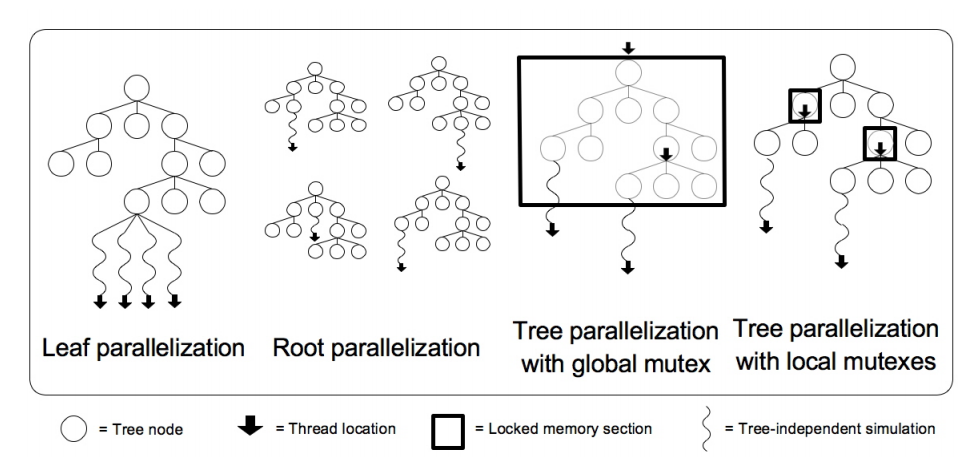
\includegraphics[scale=0.60]{2_State_of_the_art/Strategy_of_root_parallelization_Mikail/impara.png}}
   \caption{\label{étiquette} Comparison of all trees}
\label{comp_algo}
\end{figure}

Currently, the best strategy to adopt is the Root parallelization on those specific test conditions. According to some tests \cite{parallel_comp,tree_root_comp}, the advantages of the Root parallelization outcomes its drawbacks. Indeed, for 16 threads, a program using Root Parallelization will win 56\% of the time against 36.5\% for the Leaf parallelization, and 49\% for the Tree parallelization with the use of a virtual loss. Moreover, the Root is always twice faster than the Tree with virtual loss. We can explain that by the fact that numerous trees are massive, and so, you will lose much time doing communication and synchronization. You don’t have any of those problems with the Root strategy. Furthermore, this method is also very simple to compute.

\subsection{Hybrid Algorithms}

Now, we can wonder if there is some research which has already be done on hybrids technologies of parallelization. Some parallelization strategies are a combination of multiples methods with some additional content, but they are very complex to compute and are efficient in specific case.

\subsubsection{UCT-Treesplit}

The UCT-Treesplit algorithm\cite{treesplit} retakes the base of Root algorithm and add to it work clusters on which compute nodes can process. It is depicted in figure \ref{treesplit}. It’s made for High-Performance Computers (or HPC) which have cluster parallelization and shared memory parallelization. Moreover, this method demands a lot of communication and so, the network latency is a very important factor of slow-down.

\begin{figure}[!h] 
\centerline{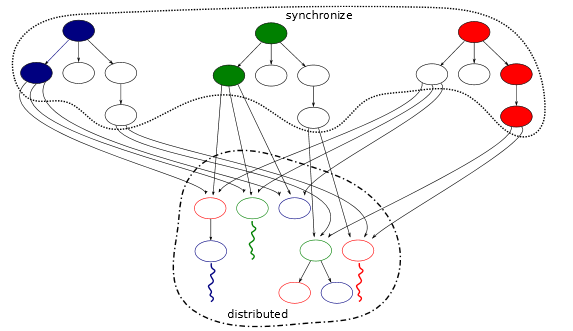
\includegraphics[scale=0.60]{2_State_of_the_art/Strategy_of_root_parallelization_Mikail/treesplit.png}}
   \caption{\label{étiquette} UCT-Treesplit scheme}
\label{treesplit}
\end{figure}

\subsubsection{Block Parallelization}

Another hybrid algorithm that is efficient is the Block Algorithm\cite{GPU}.  It is depicted in figure \ref{block}. It's working by giving some instructions to GPUs and some other instructions to CPUs. The Block Parallelization is a blending of Leaf Algorithm and Root Algorithm. As GPUs can run hundred of threads, it is used to develop a specific node with Leaf strategy whereas CPU is used to develop the trees using the Root strategy.The benefit of this method is that more since each of these components are used in the way they have been made for.

\begin{figure}[!h] 
\centerline{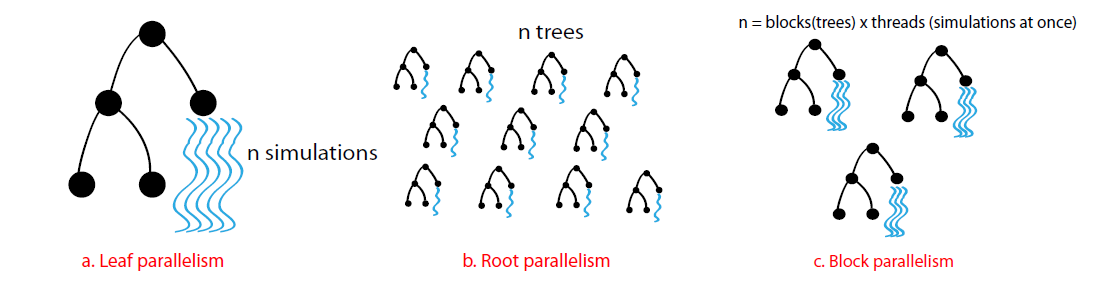
\includegraphics[scale=0.60]{2_State_of_the_art/Strategy_of_root_parallelization_Mikail/block.png}}
   \caption{\label{étiquette} Scheme of the Block Parallelization comparing to Leaf and Root}
\label{block}
\end{figure}

\subsection{Conclusion}

The strategy we will use to parralelize our algorithm depends on the hardware we will use. Since we will use both cluster parallelization and shared memory parallelization, we can choose a simple Root parallelization between the different computers, and them, use another algorithm, specialized in shared memory parallelization, like Tree Parallelization. If we prefer to use GPU instead of CPU or even both of them, we can use the Block Parallelization. Also, if our network is fast and our computers fast we can use UCT-Treesplit to parallelize our algorithm. We just have to choose what's best for our configuration.s
